\documentclass[10pt,fleqn]{article} % Default font size and left-justified equations
\usepackage{import}
\usepackage{subcaption}
\usepackage[%
    pdftitle={Energie et puissance d'un smartphone},
    pdfauthor={Geoffrey Vaquette}]{hyperref}
\subimport{../../../../style/}{preambule}
%\fichetrue
\fichefalse

%\proftrue
\proffalse

\tdtrue
%\tdfalse

\courstrue
%\coursfalse

\subimport{../../../../style/}{new_style}
\subimport{../../../../style/}{macros_SII}
\subimport{../../../../style/}{preambule_trou}

\usepackage{siunitx}
% -------------------------------------
% Déclaration des titres
% -------------------------------------

\def\discipline{Enseignement \\Technologique \\ Transversal}
\def\xxtete{Enseignement Technologique Transversal}

\def\classe{1 STI2D}
\def\xxnumpartie{Séquence 2}
\def\xxpartie{}

\def\xxnumchapitre{Séance 3}
\def\xxchapitre{\hspace{.12cm} Nombres binaires}

\def\xxposongletx{2}
\def\xxposonglettext{1.45}
\def\xxposonglety{23}
\def\xxonglet{Seq. 2 -- DS 1}

\def\xxactivite{DS}
\def\xxauteur{\textsl{Geoffrey Vaquette}}

\def\xxcompetences{%
\textsl{%
\textbf{Savoirs et compétences :}
\begin{itemize}[label=\ding{112},font=\color{ocre}]
\item CO9sin2 : Mettre en oeuvre la chaîne d’acquisition puis acquérir, \textbf{traiter, transmettre et restituer l’information}
\end{itemize}
%
}}

\def\xxfigures{
\begin{center}
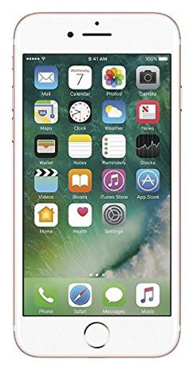
\includegraphics[height=4cm]{images/smartphone.png} \\
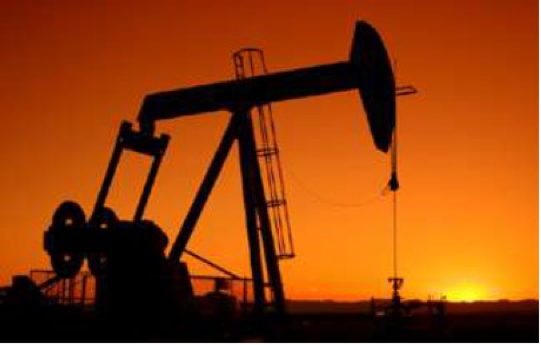
\includegraphics[height=4cm]{images/petrole.png} \\
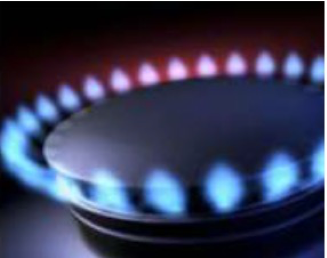
\includegraphics[height=4cm]{images/gaz.png} \\
\end{center}
}%figues de la page de garde
\def\xxpied{%
 \xxactivite%
}

%---------------------------------------------------------------------------

\renewcommand{\RemplirTrou}{true}
\begin{document}
\title{Devoir surveillé : Etude de la détection d'une ligne sur le robot moway}
\date{5 Novembre 2018}
\maketitle
\chapterimage{png/Fond_solaire}

\begin{obj}
L'objectif de ce devoir est d'évaluer votre niveau de compétence pour la compétence CO9sin2 : Mettre en oeuvre la chaîne d’acquisition puis acquérir,\textbf{ traiter, transmettre et restituer l’information. }

Nous nous intéresserons principalement à l'acquisition et à la restitution de l'information. 
 
\end{obj}

Le robot MoWay est un robot que vous avez déjà utilisé en TD/TP. C'est un robot simulant un véhicule autonome extrèmement simplifié.

Ce robot autonome peut notamment se déplacer en suivant une ligne au sol. Dans le cas classique, cette ligne est de couleur noire sur fond blanc afin d'être détectée facilement. 

Nous nous intéresserons dans ce devoir à la détection de la ligne au sol. 
Le robot moWay est équipé d'un détecteur d'obstacle situé à l'avant. C'est un capteur CNY70 de Vishay. Il donne en sortie une tension représentant la nuance (clair ou foncé) de la surface devant laquelle il est placé. 

\begin{figure}[ht]
    \centering
    \begin{subfigure}[b]{.45\textwidth}
        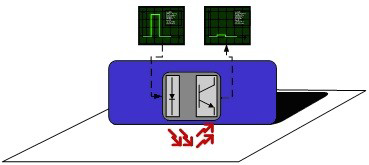
\includegraphics[width=\textwidth]{images/capteur_clair-ConvertImage.png}
        \caption{Détecteur d'obstacle placé devant une surface claire}
    \end{subfigure}
    \begin{subfigure}[b]{.45\textwidth}
        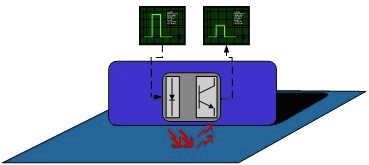
\includegraphics[width=\textwidth]{images/capteur_fonce-ConvertImage.png}
        \caption{Détecteur d'obstacle placé devant une surface grise}
    \end{subfigure}
    
    \begin{subfigure}[b]{.5\textwidth}
        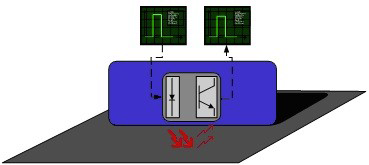
\includegraphics[width=\textwidth]{images/capteur_obscur-ConvertImage.png}
        \caption{Détecteur d'obstacle placé devant une surface obscure}
    \end{subfigure}
    
    \caption{Réaction du capteur de ligne face à différentes surfaces.}
    \label{fig:surfaces}
\end{figure}
\paragraph{}
La Figure~\ref{fig:surfaces} illustre le comportement du capteur face à différentes couleurs de surface. 

En résumé : 

\begin{description}
\item[Lorsque la surface est claire : ] La tension en sortie du capteur est \textbf{faible (minimale)} $ U = \SI{0}{V}$.
\item[Plus la surface est foncée, ] plus la tension en sortie du capteur est \textbf{forte}
\item[Lorsque la surface est noire, ] la tension en srtie du capteur est \textbf{maximale}, $U = \SI{5}{V}$. 
\end{description}

Cette tension est ensuite convertie en un \textbf{nombre binaire} sur 8 bits (un octet). Lorsque la tension est nulle, tous les bits du mot binaire sont égaux à 0. Lorsque la tension est maximale (\SI{5}{V}), tous les bits du mot binaire sont égaux à 1. 
\pagebreak
\section{Généralités}
\begin{figure}[h]
    \centering
    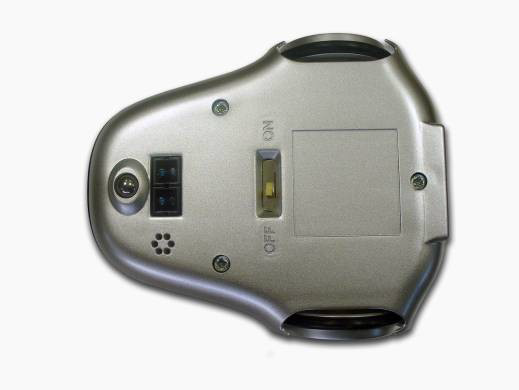
\includegraphics[width=.4\textwidth]{images/CapteurDeLigne-ConvertImage.png}
    \caption{Position du capteur de ligne sur le moway}
    \label{fig:moway}
\end{figure}

\begin{exercise}
    \begin{question}
        Sur la Figure~\ref{fig:moway}, entourez la localisation du capteur de luminosité. 
    \end{question}
\end{exercise}


\section{Valeurs extrêmes du capteur}
\begin{exercise}~
\begin{question}
  A partir des informations ci-dessus donnez, en justifiant, les valeurs binaires lorsque la surface est blanche. 
\end{question}
\begin{question}
  Même question lorsque la surface est totalement noire. 
\end{question}
\begin{question}
  Convertissez les deux valeurs binaires précédentes dans le domaine décimal (détaillez les calculs). 
\end{question}
\end{exercise}

\section{Conversion binaire - décimal - binaire}

Lorsque la couleur du sol varie, les valeurs en entrée du processeur varient de $0_{(10)}$ à $255_{(10)}$. Nous proposons dans cette partie de convertir diverses valeurs de niveau de gris en valeurs binaires. 


\begin{exercise}~

\begin{question}
Convertissez les valeurs suivantes du domaine décimal vers binaire en utilisant au moins une fois la méthode par soustraction et au moins une fois la méthode par division et en détaillant les calculs : 
  \begin{itemize}
      \item $122_{(10)} = \dots~_{(2)}$
      \item $13_{(10)} = \dots~_{(2)}$
      \item $319_{(10)} = \dots~_{(2)}$
      \item $253_{(10)} = \dots~_{(2)}$
  \end{itemize}
\end{question} 


\begin{question}
A l'inverse, convertissez les valeurs binaires suivantes dans le domaine décimal : 
\begin{itemize}
    \item $1001~0111 _{(2)}  = \dots~_{(10)}$
    \item $0001~0100 _{(2)}  = \dots~_{(10)} $
    \item $1101~0001 _{(2)} = \dots~_{(10)} $
    \item $1110~1101 _{(2)} = \dots~_{(10)} $
\end{itemize}
\end{question}

\begin{question}
Convertissez les valeurs binaires suivantes dans le domaine hexadécimal : 
\begin{itemize}
    \item $1001~0111 _{(2)}  = \dots~_{(16)}$
    \item $0001~0100 _{(2)}  = \dots~_{(16)} $
    \item $1101~0001 _{(2)} = \dots~_{(16)} $
    \item $1110~1101 _{(2)} = \dots~_{(16)} $
\end{itemize}
\end{question}
\end{exercise}


\end{document}